\documentclass[sensors,article,submit,moreauthors, xelatex]{Definitions/mdpi} 

%=================================================================
\firstpage{1} 
\makeatletter 
\setcounter{page}{\@firstpage} 
\makeatother
\pubvolume{xx}
\issuenum{1}
\articlenumber{5}
\pubyear{2019}
\copyrightyear{2019}
%\externaleditor{Academic Editor: name}
\history{Received: date; Accepted: date; Published: date}
%\updates{yes} % If there is an update available, un-comment this line

%% MDPI internal command: uncomment if new journal that already uses continuous page numbers 
%\continuouspages{yes}

%------------------------------------------------------------------
% The following line should be uncommented if the LaTeX file is uploaded to arXiv.org
%\pdfoutput=1

%=================================================================
% Add packages and commands here. The following packages are loaded in our class file: fontenc, calc, indentfirst, fancyhdr, graphicx, lastpage, ifthen, lineno, float, amsmath, setspace, enumitem, mathpazo, booktabs, titlesec, etoolbox, amsthm, hyphenat, natbib, hyperref, footmisc, geometry, caption, url, mdframed, tabto, soul, multirow, microtype, tikz
\usepackage[acronym, nogroupskip, nonumberlist]{glossaries}

\setglossarystyle{long}
\renewenvironment{theglossary}%
  {\begin{longtable}[l]{l l p{\glsdescwidth}}}
  {\end{longtable}}
 
\makenoidxglossaries
\newacronym{roi}{ROI}{region of interest}
\newacronym{sfm}{SfM-MVS}{Structure-from-Motion Multi-View Stereo photogrammetry}
\newacronym{dom}{DOM}{digital orthophoto map}
\newacronym{dsm}{DSM}{digital surface model}
\newacronym{lidar}{LiDAR}{light detection and ranging}
\newacronym{ml}{ML}{machine learning}
\newacronym{dl}{DL}{deep learning}

%=================================================================
%% Please use the following mathematics environments: Theorem, Lemma, Corollary, Proposition, Characterization, Property, Problem, Example, ExamplesandDefinitions, Hypothesis, Remark, Definition, Notation, Assumption
%% For proofs, please use the proof environment (the amsthm package is loaded by the MDPI class).

%=================================================================
% Full title of the paper (Capitalized)
\Title{EasyRIC: A post process tool for }

% Author Orchid ID: enter ID or remove command
\newcommand{\orcidauthorA}{0000-0001-6135-402X} % Add \orcidA{} behind the author's name
%\newcommand{\orcidauthorB}{0000-0000-000-000X} % Add \orcidB{} behind the author's name

% Authors, for the paper (add full first names)
\Author{Haozhou Wang $^{1}$\orcidA{} and Wei Guo $^{1}$*}
% special signal: \dagger,\ddagger in $$ parts

% Authors, for metadata in PDF
\AuthorNames{Haozhou Wang and Wei Guo}

% Affiliations / Addresses (Add [1] after \address if there is only one affiliation.)
\address[1]{
%$^{1}$ \quad Affiliation 1; e-mail@e-mail.com\\
%$^{2}$ \quad Affiliation 2; e-mail@e-mail.com
$^{1}$ \quad International Field Phenomics Research Laboratory, Institute for Sustainable Agro-ecosystem Services, Graduate School of Agricultural and Life Science, The Univerisity of Tokyo, Japan.
}

% Contact information of the corresponding author
\corres{Correspondence: guowei@g.ecc.u-tokyo.ac.jp}%; Tel.: (optional; include country code; if there are multiple corresponding authors, add author initials) +xx-xxxx-xxx-xxxx (F.L.)}

% Current address and/or shared authorship
%\firstnote{Current address: Affiliation 3} 
%\secondnote{These authors contributed equally to this work.}
% The commands \thirdnote{} till \eighthnote{} are available for further notes

%\simplesumm{} % Simple summary

%\conference{} % An extended version of a conference paper

% Abstract (Do not insert blank lines, i.e. \\) 
\abstract{Applying high-throughput phenotyping technologies in agriculture provides an advanced and efficient method for managing and breeding crops in practical applications. Compared with device-specified remote sensing technologies (laser scanning, \acrfull*{lidar}, etc.), \acrfull*{sfm}, applicable to price friendly RGB digital cameras, has been widely spread use around the world, and many commercial and open-source software are available to implement this task. However, producing good quality of its products, such as \acrfull*{dom}, \acrfull*{dsm}, and point clouds, is quite computation intensive and hard to meet the same precision of original photos. Hence, linking low computation time produced low quality \acrshort*{sfm} products back to original digital images has significant potential to improve the efficiency and precision for data processing, but to the best of our knowledge, no easy-to-use open source tool is available for this object. In this study, a pure python package called EasyRIC (easy reconstruction image converter) was developed to link original photos to \acrshort*{sfm} products. The Lotus (\textit{Nelumbo nucifera}) breeding field were used as a show case to demonstrate the following functions: 1) Clipping the \acrfull*{roi} from point clouds and compare them throught time series. 2) Clipping the \acrshort*{roi} from \acrshort*{sfm} products to raw images. 3) Generate bunch of training data in raw images from a few manual marked \acrshort*{roi}. This python package shows the great potential to integrate the high-quality original images with  \acrshort*{sfm} produced products. The quick produced low quality products are also acceptable which saved plenty computation time. Also this tool can be used to generate bunch of training data for machine learning with a few manual operation.}

% Keywords
\keyword{3D reconstruction, Orthomosaic, Training data generation, Phenotyping, Open source, Pix4D}

%+++++++++++++++++++++++++++++++++++++++++++++++++++++++++

\begin{document}

\section{Introduction}
Para1: Agricultural crisis -> demand for high-throughput phenotyping

Para2: Common high-throughput phenotyping technologies -> why RGB SfM

Para3: SfM background, \textbf{algorithm}, and software (computation intensive drawbacks, need low quality to save time)

Para4: Data processing (the difficulties to of use the result of SfM, e.g. 1) low quality of DOM make canopy cover, organ detection. -> link to raw image; 2) 3D analysis not easy (require large RAM and good computation to processing point cloud, and the quality of point cloud couldn't too large -> 3D to 2d, 3D clipping, there is no common tool to make this transfer easy)

Para5: 4D time series analysis demand and point cloud clipping

Para6: Training Data crisis

Para7: Objectives

\section{Methods and Materials}

\subsection{Experimental design}
Experimental design about Lotus (Figure  \ref{fig:plotid}), (in order to test this package, the following data were collected, and SfM products were produced by the following configs, using Pix4D as an exmaple)

\begin{figure}[H]
\centering
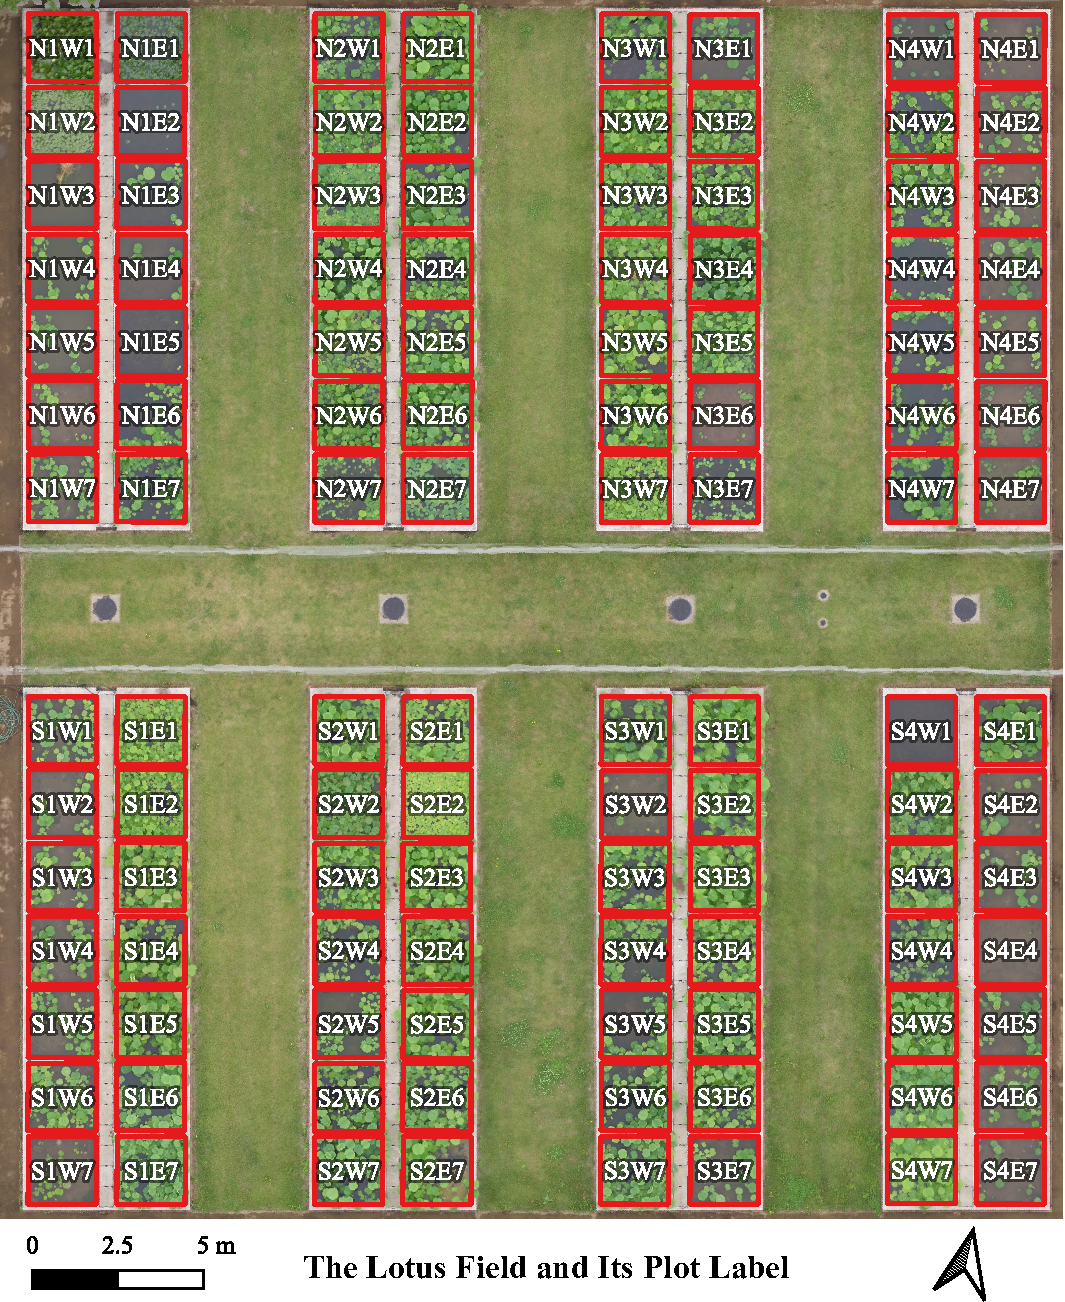
\includegraphics[width=0.95\linewidth]{figures/plot_with_id.pdf}
\caption{Lotus plot id. localtion: Tokyo, Japan, DOM, 2017.05/09 made by QGIS, including this figure and label shapefile (shp), This need to be modified later}
\label{fig:plotid}
\end{figure}

\subsection{Data collection}
\subsubsection{Instruments}

\subsubsection{\acrshort*{sfm} configuration}
It is quite important to ensure the quality of input data is analysiable. This part introduce the method about how to prepare raw images and \acrshort*{sfm} outputs. 

Ground control points, flight speed etc.

\subsection{Implementation}
The definition of each camera external parameters and 2D \& 3D coordinates

\subsubsection{Software workflow}
Show the workflow chart 

\begin{figure}[H]
\centering
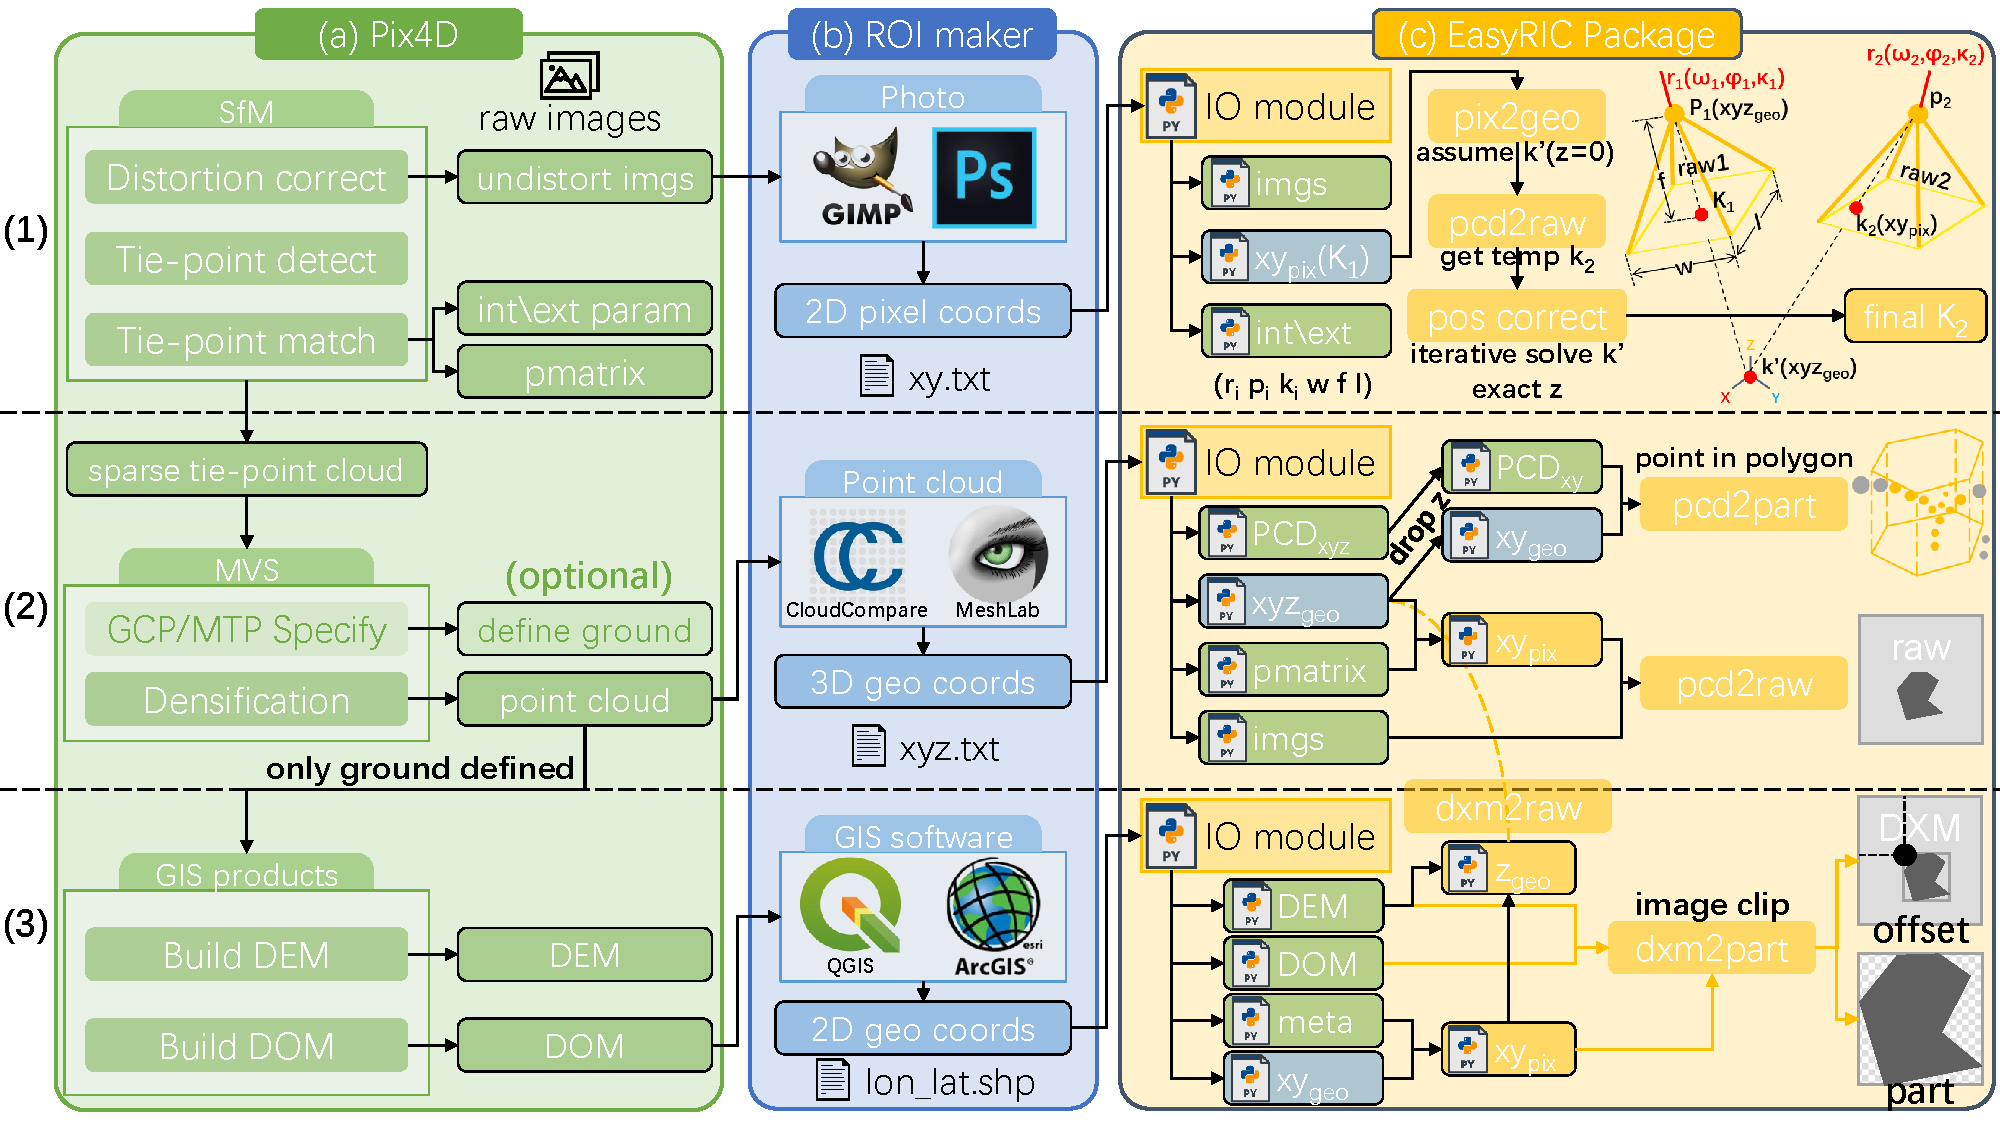
\includegraphics[width=0.95\linewidth]{figures/workflow.pdf}
\caption{Workflow of software. This need to be modified later}
\end{figure}

%\begin{figure}[H]
%\centering
%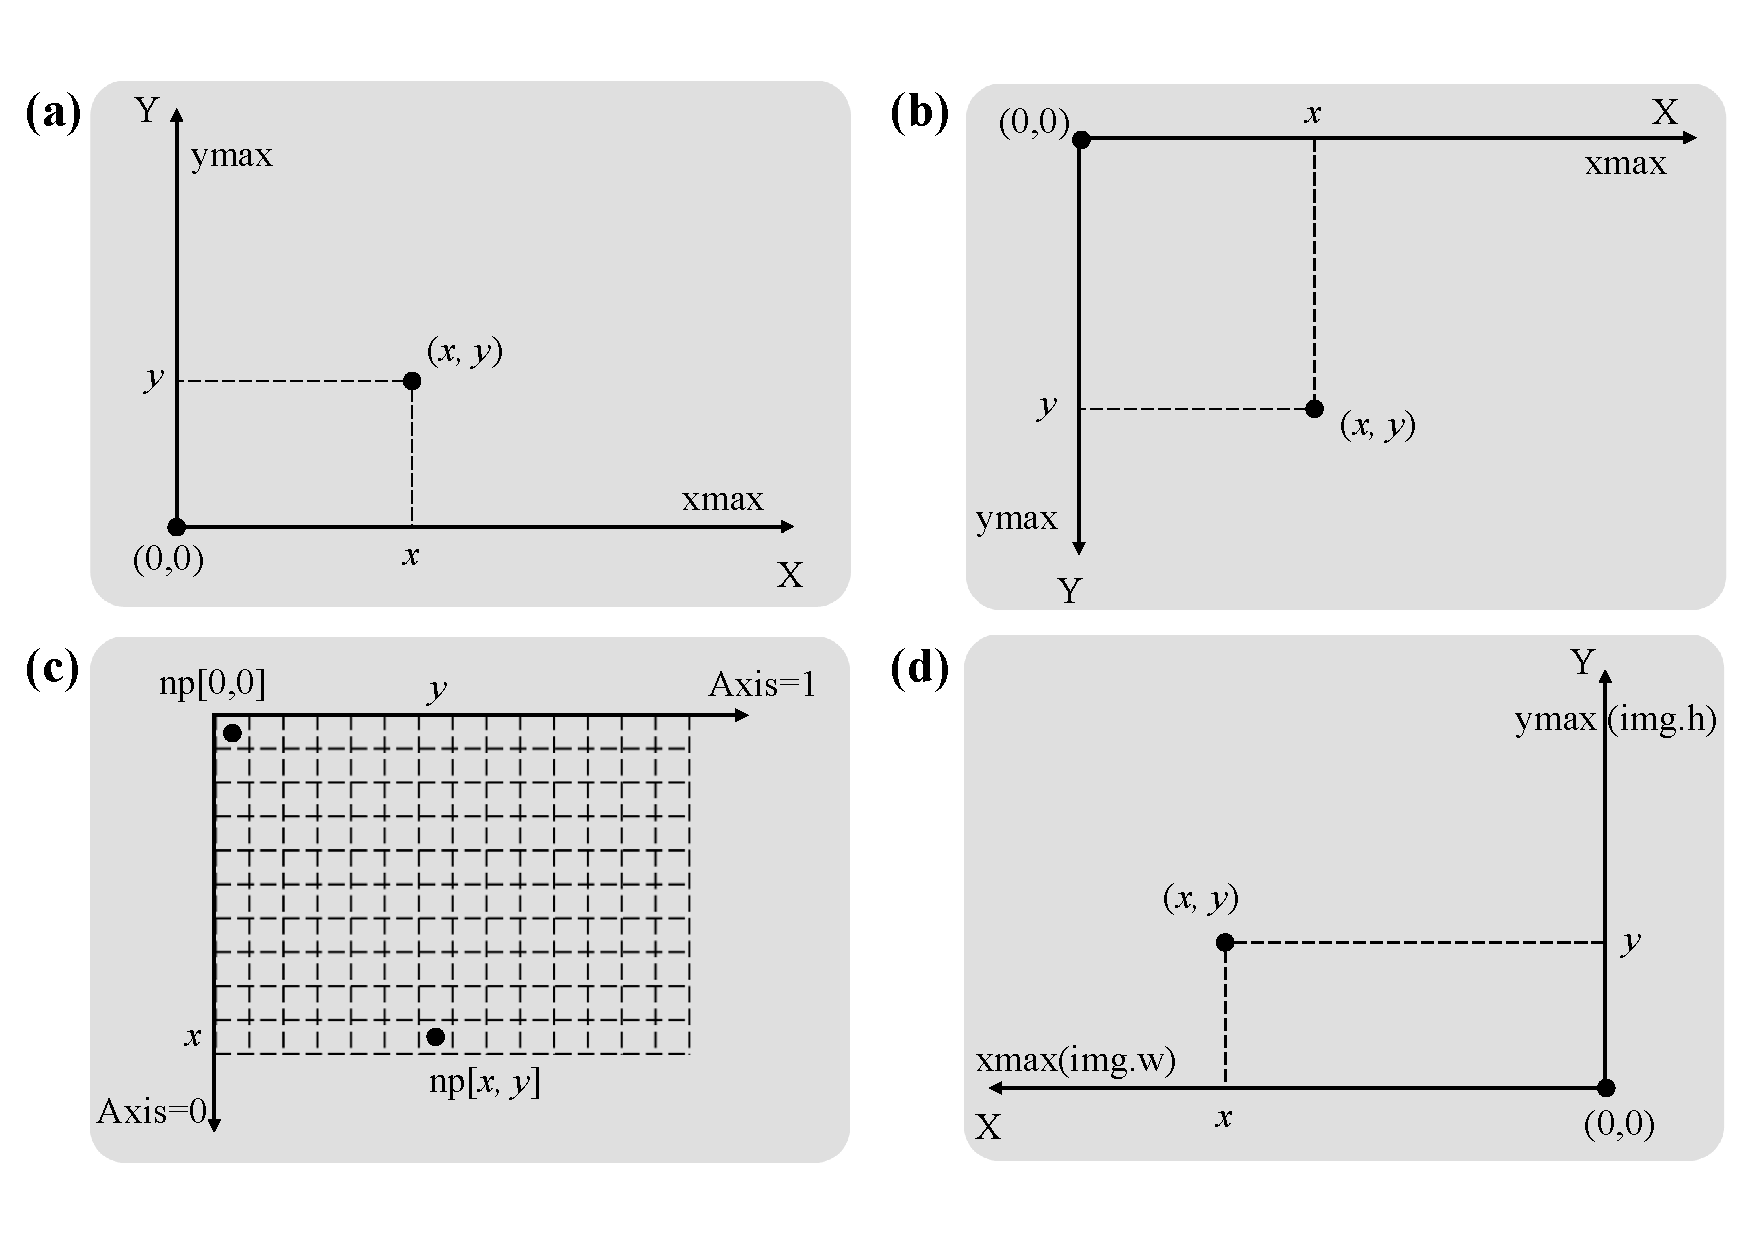
\includegraphics[width=0.95\linewidth]{figures/coordinates.pdf}
%\caption{The coordinates used. This need to be modified later, add 3D into it}
%\end{figure}

\subsubsection{Conversion algorithms}
1) from 2D Photo pixel coordinate to 2D Geo coordinate (DOM DSM, via GeoTiff header info)

2) 2D Geo coordinate to 3D Geo coordinate (Point clouds) via DSM (know xy, search z from DSM)

3) 3D Geo coordinate projects to 2D pixel coordinate via camera parameters from SfM output

4) [Future work] 2D photo pixel to 3D Geo coordinate without GIS information, using Shi Yun's algorithm, (not sure mention in this part or future work part)

%\subsection{Software dependency}
Python packages, platforms (Windows for exe)

Pix4D OpenSFM, FieldReconst (http://cse.naro.affrc.go.jp/rsugiura/FieldReconst/) introduction

%\subsection{Hardware dependency}
"\textit{For reliable performance of the system, server specifications of 8 GB of RAM and a multicore CPU with at least 3 GHz are recommended. The web-application can be accessed by any connected smart device capable of
running standard web-browsers.}" (copied from another software paper, need modification)

\subsubsection{Software operations}
Python command and classes to do previous workflow

Also introduce GUI interface (CMD line) if we have.

\section{Results}

\subsection{Use case 1: Point cloud segmentation}
Compare \acrshort*{roi} by time series

In this part, both raw photo? DOM? and point clouds should be displayed? Clipping point clouds may requires Open3D packages, which can not guarantee easy to be packed up.

\subsection{Use case 2: plot segmentation}

Find \acrshort*{roi} in \acrshort*{sfm} products on the raw images

text \cite{ma_calculation_2019, guo_illumination_2013}
should including from DOM(DSM) coordinates (GIS or pixel) and point clouds (3D) coordinates to raw images.

\subsection{Use case 3: Efficient annotation of training data for \acrshort*{ml}/\acrshort*{dl}}
3D/2.5D small region -> 2D->Raw small region, selecting strategy for efficient annotation of training data for ML/DL.

\section{Discussion}

%\subsection{Future prospects}
API for most \acrshort*{sfm} software packages

2D Photo to 2D photo without SfM products

Link between Aerial and Terristrial photos.

\section{Conclusions}
Text

%%%%%%%%%%%%%%%%%%%%%%%%%%%%%%%%%%%%%%%%%%
\vspace{6pt} 

%\section{Availability and requirements}
%\begin{itemize}
%  \item \textbf{Project name:} EasyRIC
%  \item \textbf{Project home page:} https://github.com/HowcanoeWang/EasyRIC
%  \item \textbf{Operating system(s):} Using the source codes as Python package is platform independent, also providing executable software package for windows (windows 10 and 64-bit is tested and recommended).
%  \item \textbf{Programming language: } Python
%  \item \textbf{Other requirements:} For using source code as package: Python 3.7 or higher, numpy 1.18.1 or higher, scikit-image 0.16.2 or higher; For using executable software packages on Windows, 64-bit windows is required, and Intel CPU (with mkl support) is recommended.
%  \item \textbf{License:} GPL-3.0
%  \item \textbf{Any restrictions to use by non-academics:} Free to use for any purpose, forever.
%\end{itemize}

%%%%%%%%%%%%%%%%%%%%%%%%%%%%%%%%%%%%%%%%%%
\authorcontributions{For research articles with several authors, a short paragraph specifying their individual contributions must be provided. The following statements should be used ``conceptualization, X.X. and Y.Y.; methodology, X.X.; software, X.X.; validation, X.X., Y.Y. and Z.Z.; formal analysis, X.X.; investigation, X.X.; resources, X.X.; data curation, X.X.; writing--original draft preparation, X.X.; writing--review and editing, X.X.; visualization, X.X.; supervision, X.X.; project administration, X.X.; funding acquisition, Y.Y.'', please turn to the  \href{http://img.mdpi.org/data/contributor-role-instruction.pdf}{CRediT taxonomy} for the term explanation. Authorship must be limited to those who have contributed substantially to the work reported.}

%%%%%%%%%%%%%%%%%%%%%%%%%%%%%%%%%%%%%%%%%%
\funding{Please add: ``This research received no external funding'' or ``This research was funded by NAME OF FUNDER grant number XXX.'' and  and ``The APC was funded by XXX''. Check carefully that the details given are accurate and use the standard spelling of funding agency names at \url{https://search.crossref.org/funding}, any errors may affect your future funding.}

%%%%%%%%%%%%%%%%%%%%%%%%%%%%%%%%%%%%%%%%%%
\acknowledgments{In this section you can acknowledge any support given which is not covered by the author contribution or funding sections. This may include administrative and technical support, or donations in kind (e.g., materials used for experiments).}

%%%%%%%%%%%%%%%%%%%%%%%%%%%%%%%%%%%%%%%%%%
\conflictsofinterest{Declare conflicts of interest or state ``The authors declare no conflict of interest.'' Authors must identify and declare any personal circumstances or interest that may be perceived as inappropriately influencing the representation or interpretation of reported research results. Any role of the funders in the design of the study; in the collection, analyses or interpretation of data; in the writing of the manuscript, or in the decision to publish the results must be declared in this section. If there is no role, please state ``The funders had no role in the design of the study; in the collection, analyses, or interpretation of data; in the writing of the manuscript, or in the decision to publish the results''.} 

%%%%%%%%%%%%%%%%%%%%%%%%%%%%%%%%%%%%%%%%%%
%% optional
%\abbreviations{The following abbreviations are used in this manuscript:\\

%\noindent 
%\begin{tabular}{@{}ll}
%MDPI & Multidisciplinary Digital Publishing Institute\\
%DOAJ & Directory of open access journals\\
%TLA & Three letter acronym\\
%LD & linear dichroism
%\end{tabular}}

%\renewcommand*{\glsgroupskip}{}
\printnoidxglossary[type=\acronymtype, title=Abbreviations]

%%%%%%%%%%%%%%%%%%%%%%%%%%%%%%%%%%%%%%%%%%
%% optional
%\appendixtitles{no} %Leave argument "no" if all appendix headings stay EMPTY (then no dot is printed after "Appendix A"). If the appendix sections contain a heading then change the argument to "yes".
%\appendix
%\section{}
%\unskip
%\subsection{}
%The appendix is an optional section that can contain details and data supplemental to the main text. For example, explanations of experimental details that would disrupt the flow of the main text, but nonetheless remain crucial to understanding and reproducing the research shown; figures of replicates for experiments of which representative data is shown in the main text can be added here if brief, or as Supplementary data. Mathematical proofs of results not central to the paper can be added as an appendix.

%\section{}
%All appendix sections must be cited in the main text. In the appendixes, Figures, Tables, etc. should be labeled starting with `A', e.g., Figure A1, Figure A2, etc. 

%%%%%%%%%%%%%%%%%%%%%%%%%%%%%%%%%%%%%%%%%%
% Citations and References in Supplementary files are permitted provided that they also appear in the reference list here. 
\reftitle{References}
%=====================================
% References, variant B: external bibliography
%=====================================
\externalbibliography{yes}
\bibliography{myzotero}

%%%%%%%%%%%%%%%%%%%%%%%%%%%%%%%%%%%%%%%%%%
%% optional
%\sampleavailability{Samples of the compounds ...... are available from the authors.}

%% for journal Sci
%\reviewreports{\\
%Reviewer 1 comments and authors’ response\\
%Reviewer 2 comments and authors’ response\\
%Reviewer 3 comments and authors’ response
%}

%%%%%%%%%%%%%%%%%%%%%%%%%%%%%%%%%%%%%%%%%%
\end{document}
